\documentclass[11pt,a4paper]{article}

\usepackage[utf8]{inputenc}
\usepackage[T1]{fontenc}
\usepackage{lmodern}
\usepackage{textcomp}
\usepackage{amsmath,amssymb}
\usepackage{algorithm}
\usepackage{algpseudocode}
\usepackage{booktabs}
\usepackage[authoryear,round]{natbib}
\usepackage{hyperref}
\usepackage{listings}
\usepackage{needspace}
\usepackage{etoolbox}
% A short listing must not split across a page: ask for room before it starts.
\BeforeBeginEnvironment{lstlisting}{\needspace{6\baselineskip}}
\usepackage{xcolor}
\usepackage[margin=2.5cm]{geometry}
\usepackage{enumitem}
\usepackage{graphicx}
\usepackage{tikz}
\usetikzlibrary{arrows.meta,positioning,shapes.geometric,calc,fit,backgrounds}
\setlength{\parskip}{0.4em}
\setlength{\parindent}{0em}

\hypersetup{
    colorlinks=true,
    linkcolor=blue!60!black,
    citecolor=blue!60!black,
    urlcolor=blue!60!black
}

\definecolor{codebg}{HTML}{F5F5F5}

\tikzset{
    diag title/.style={font=\sffamily\small\bfseries},
    diag box/.style={
        draw=black!75,
        rounded corners=1.5pt,
        fill=gray!4,
        minimum height=0.82cm,
        minimum width=2.5cm,
        align=center,
        font=\sffamily\small,
        inner sep=4pt
    },
    diag data/.style={diag box, rounded corners=0.5pt, fill=gray!8},
    diag ai/.style={diag box, rounded corners=4pt, fill=gray!11},
    diag det/.style={diag box, rounded corners=0.5pt, fill=gray!12, line width=1.0pt},
    diag out/.style={diag box, fill=white},
    diag header/.style={diag box, fill=gray!10, font=\ttfamily\small},
    diag decision/.style={
        draw=black!75,
        diamond,
        aspect=2.35,
        fill=white,
        inner sep=2pt,
        align=center,
        font=\sffamily\scriptsize
    },
    diag terminal/.style={
        draw=black!75,
        rounded corners=1.5pt,
        fill=gray!2,
        minimum height=0.7cm,
        minimum width=1.95cm,
        align=center,
        font=\sffamily\scriptsize\bfseries,
        inner sep=4pt
    },
    diag code/.style={font=\ttfamily\scriptsize, align=left},
    diag note/.style={font=\sffamily\scriptsize, text=black!70, align=center},
    diag label/.style={font=\sffamily\scriptsize, text=black!60},
    diag arrow/.style={-{Stealth[length=4pt]}, semithick, draw=black!70},
    diag feedback/.style={-{Stealth[length=4pt]}, dashed, semithick, draw=black!60}
}

% TeX widens the space after a colon (space factor 2000), which turned the
% inline code "?[r: IS_AT_RISK]" into "?[r:  IS_AT_RISK]". A colon is not the
% end of a sentence here, so give it the plain space factor everywhere.
\sfcode`\:=1000

\lstset{
    upquote=true,
    basicstyle=\small\ttfamily,
    backgroundcolor=\color{codebg},
    frame=single,
    framerule=0.5pt,
    rulecolor=\color{gray!30},
    breaklines=true,
    columns=flexible,
    keepspaces=true,
    tabsize=2
}


\title{\textbf{ProveML: Inline Claim Markup for Deterministic Verification of AI-Generated Text}}
\author{Shane Deconinck\\\small{abovebeyond.ai}\\\small{\texttt{hello@shanedeconinck.be}}}
\date{August 2026}

\begin{document}

\maketitle

\begin{abstract}
Organizations are deploying LLMs in consequential settings~\citep{aiindex2026,magesh2025}, and regulation now reaches generated text~\citep{euaiact,art50guidelines2026}, but the text seldom carries a link between an individual claim and the data behind it that a machine can check~\citep{citednotverified,rao2026}. We present ProveML, a Markdown extension of three inline constructs that places AI-generated claims inside a verifiable boundary: the constructs declare entities, link facts to a data source, and check qualitative judgments against pre-declared thresholds. Verification is deterministic, string equality and numeric comparison against a flat key-value store with no model in the loop, so it is explainable, costs milliseconds per response, can sit inside a generation loop that feeds each error back to the model, and can audit text it did not generate; its semantics is stated formally and its guarantees, that verified means equal to the store and that no unregistered name can decide a judgment, are proven in a mechanised model. The verifier also reports coverage: the share of the numbers in a text that sit inside a claim at all. We evaluate three frontier models of August 2026 (Claude Opus 5, Claude Sonnet 5 and DeepSeek V4 Pro) on a generated educational benchmark and real SEC EDGAR filings, three runs each with one correction pass. All three produce the markup on every query, put 90--96\% of their numbers inside a claim, and verify 87--100\% of those claims on the first pass and 92--100\% after one correction. Given a registry of fourteen named conditions, all three make their qualitative judgments through it, never name a condition it does not hold, and verify 78--100\% of those judgments on the first pass and 98--100\% after one correction; the failures are the word the question invited, refused by the bound. Most residual errors come from one binding rule, a fact attaching to the nearest entity; making the remedy part of the specification, a fact may name its own record, lifts first-pass verification to 95--100\%. The specification, verifier, benchmarks and all run artifacts are published.
\end{abstract}

\noindent\textbf{Keywords:} AI verification, markup language, deterministic verification, structured data, threshold registry, hallucination detection, inline tagging


\section{Introduction}

Large Language Models (LLMs) produce fluent, contextually appropriate text that untrained readers can no longer reliably distinguish from human-authored content \citep{clark2021,jakesch2023,jones2026}; readers who write with these models daily still can \citep{russell2025}. The fluency carries no reliable signal of the model's own uncertainty: deployed models rarely volunteer uncertainty even when they are wrong, verbalised confidence is systematically overconfident, and the training pipeline rewards a confident guess over an admission of ignorance \citep{zhou2024,xiong2024,kalai2025}. And the fluency coexists with a fundamental reliability problem: \textbf{LLMs hallucinate} \citep{ji2023}. They generate text that is plausible but factually incorrect: fabricated citations, 3--13\% of the citation URLs supplied by commercial models and deep research agents in 2026 having never existed \citep{rao2026}; numbers with no basis in the source \citep{cao2024}; and statements whose citations do not support them \citep{liu2023verifiability}.

Hallucination is structural, not incidental: calibrated language models must hallucinate at a rate approaching the fraction of facts appearing exactly once in training \citep{kalai2024}, and standard training pipelines reward guessing over acknowledging uncertainty \citep{kalai2025}. Regulation no longer adds urgency; it adds exposure. The EU AI Act's transparency duties have applied since 2 August 2026, with the Commission's Article~50 guidelines adopted two weeks before; the Digital Omnibus deferred only the machine-readable marking duty for systems already on the market, to 2 December 2026 \citep{euaiact,art50guidelines2026,omnibus2026}. But the Code of Practice that operationalises these duties concerns marking the \textit{origin} of content and says nothing about its accuracy \citep{transparencycode2026}: a text can be fully compliant and wrong. And the problem has not gone away with better models: the leading legal research tools hallucinated on 17--33\% of queries when tested in 2024, despite vendor claims of near-elimination \citep{magesh2025}, and a 2026 survey of court filings found more than a thousand containing fabricated citations, a number growing year over year \citep{liu2026citations}.

The models are meanwhile in production. Generative AI is used in at least one business function at 70\% of surveyed organizations \citep{aiindex2026}, in legal research \citep{magesh2025} and in clinical documentation \citep{wright2026}. Even systems built to cite fall short: in 2026 the citations of frontier deep-research agents were factually accurate for only 39--77\% of claims, and 10.7\% of the citation URLs of the two commercial deep research agents never existed, against 4.8\% for search-augmented models \citep{citednotverified,rao2026}, three years after the first generative search engines fully supported about half of their sentences \citep{liu2023verifiability,alce}; and whether a citation holds is judged by a person or by another model rather than by a deterministic check \citep{ais,citednotverified}.

The response this paper takes is not to make the model more truthful but to make its claims \textit{checkable}: every marked claim either matches an addressable record or is flagged, deterministically, before anyone reads it. In short, \textbf{ProveML is iXBRL for AI-generated text.} Financial reporting solved a version of this problem two decades ago by embedding machine-readable tags in human-readable filings, so a regulator can audit a number without reading the prose around it \citep{ixbrl}. ProveML applies that idea where the author is a model rather than a person, and adds what that setting needs: entity scoping, so a value is bound to the record it describes, and a threshold registry, so a qualitative judgment is a declared predicate rather than a choice of adjective; Figure~\ref{fig:render-errors} shows what that buys the reader.

\begin{figure}[h]
\centering
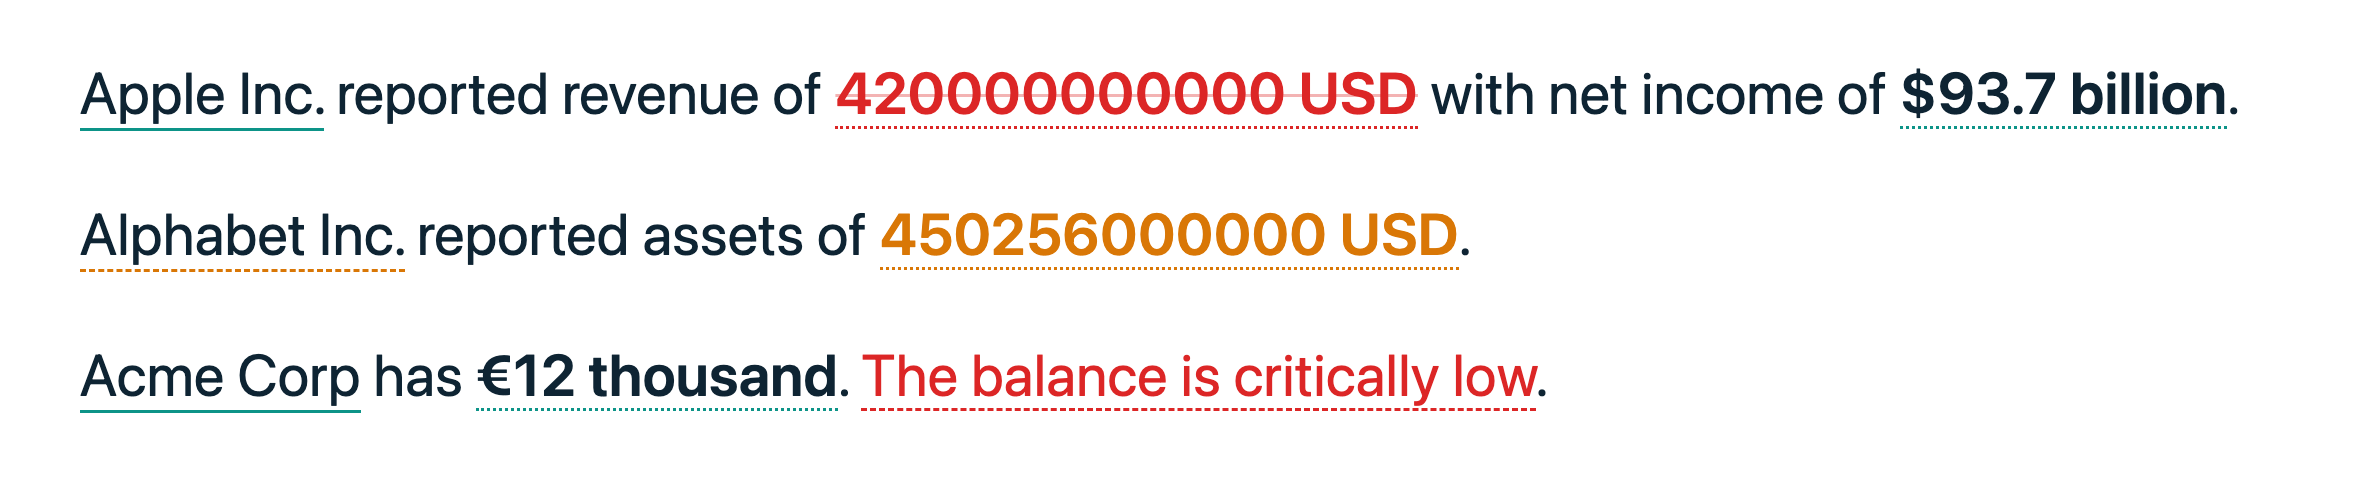
\includegraphics[width=\textwidth]{fig-verify-errors.png}
\caption{What the reader sees after verification: a wrong revenue figure struck through, a claim about a company the store does not know left open, a judgment whose condition does not hold marked as failed. The model wrote 93736000000; the store's display rule turns it into ``\$93.7 billion'' once it has verified. The wrong revenue figure never verified, so it stays as the model wrote it.}
\label{fig:render-errors}
\end{figure}

Two things decide whether ProveML fits a use. First, verification is exact: the model writes the value as the store holds it, \texttt{391035000000}, and ``\$391 billion'' in its place fails. Readability is the renderer's job, not the model's: the store declares a display rule for the field and the renderer applies it after verification (Section~\ref{sec:proveml}). That is the guarantee, and it asks for a store that holds canonical values. Second, the threshold registry is the deployment's: the names a model may use, and the bound behind each, are declared before generation, so a judgment the deployment never named cannot be made checkable by the model. Section~\ref{sec:evaluation} measures what models do with such a registry. Section~\ref{sec:limitations} gives the full list of limits.

This paper is deliberately compact: it gives the idea, the three constructs, what the mechanism costs, and what we measured on three models that were frontier in August 2026 (Claude Opus 5, Claude Sonnet 5 and DeepSeek V4 Pro). The complete specification (verification algorithm, comparison semantics, rendering) is in the accompanying technical report, together with the July 2026 study of smaller models that preceded this one, whose results this paper does not reproduce; the three-valued condition semantics is stated in Appendix~\ref{app:formal}. Both documents are published in the artifact repository alongside every benchmark, run artifact, and the scripts that regenerate every table.\footnote{\url{https://github.com/abovebeyond-ai/proveml-research} --- reference implementation: \url{https://github.com/abovebeyond-ai/proveml} (npm: \texttt{proveml}).}

\section{ProveML}
\label{sec:proveml}

ProveML extends Markdown with three constructs, using characters (\texttt{@}, \texttt{\%}, \texttt{?}) that do not conflict with standard Markdown syntax. Instruction-tuned models routinely answer in Markdown \citep{sun2025idiosyncrasies}, and a CommonMark-conformant renderer passes the constructs through unchanged, because characters not given an interpretation by any Markdown rule are parsed as plain textual content \citep{commonmark}; in our runs every model produced the markup on every query.

\begin{lstlisting}
(* Simple form: entity, then facts follow *)
@[sensor:42]{Sensor X} reads %[value]{29.99} with %[stock]{150} in stock.

(* Scoped form: facts inside entity braces *)
@[sensor:42 "Sensor X"]{reads %[value]{29.99}, %[stock]{150} in stock}

(* Nested scopes: outer entity with multiple inner entities *)
@[facility:7 "Plant North"]{hosts
  @[sensor:42 "Sensor X"]{reading %[value]{29.99}} and
  @[sensor:43 "Sensor Y"]{reading %[value]{18.5}},
  with %[sensorCount]{12} sensors total}
\end{lstlisting}

\paragraph{Entity references} \texttt{@[type:id]\{name\}} declare the subject. The verifier checks the display name against the store (\texttt{sensor:42.name}), and the entity becomes the context for the facts that follow. Binding is structural, never controlled by the LLM: a fact inside scoped braces binds to that entity (lexical scope); a fact outside binds to the last simple-form entity at the current depth (linear carry-forward), and closing a scope restores the context that was in force when it opened.

\paragraph{Fact references} \texttt{\%[field]\{value\}} claim a value. The verifier checks $\texttt{store}[\textit{entity}.\textit{field}] = \textit{value}$ by exact string equality on the store's canonical representation (the store follows below; where the store declares a unit, the claim carries it, as in \texttt{\%[balance]\{-12400 EUR\}}). Four outcomes: \textit{verified}, \textit{mismatch}, \textit{unverifiable} (no such field), \textit{no context}. A fact may also name its own record, \texttt{\%[student:20414.passRate]\{53\}}, for a sentence whose subject is not the nearest entity; Section~\ref{sec:evaluation} shows why that is needed.

\paragraph{Inference references} \texttt{?[label: CONDITION]\{text\}} make a qualitative judgment checkable. The condition names a threshold from a registry defined outside generation; the model cannot invent a comparison value, a bound, or a direction, and an unregistered name is an error rather than a claim. Conditions compose with \texttt{AND}, \texttt{OR}, \texttt{NOT} and can reference earlier labels:

\begin{lstlisting}
?[low: IS_LOW]{critically low score}
?[missing: IS_MISSING]{no recent data}
?[risk: @low AND @missing]{low score with missing data}
\end{lstlisting}

\paragraph{The fact store} is a flat key-value index in the Entity-Attribute-Value pattern \citep{nadkarni1999,dinu2007}; any source with records and fields flattens into it as \texttt{type:id.field $\rightarrow$ value}, with optional companion keys for units and nested sub-paths for hierarchical data:

\begin{lstlisting}
account:901.holder                       -> "Acme Corp"
account:901.balance                      -> -12400
account:901.balance._unit                -> "EUR"
account:901.overdue                      -> 3
account:901.transaction:2026-01.amount   -> 5200
account:901.transaction:2026-01.amount._unit -> "EUR"
\end{lstlisting}

\noindent The store is the single point of trust and the canonicalization point: the guarantee is ``consistent with the fact store'', not ``true'', and verification is always relative to an immutable store state (deployments can bind a snapshot identifier to each result). Arithmetic lives in the data layer, not the verifier: a cross-entity difference is materialized as an addressable fact (\texttt{region:EU.\_salesDiff}) and bounded by a registered predicate, so every operand of every comparison is itself auditable. So does presentation: a companion key \texttt{revenue.\_display = currency:USD:1} tells the renderer to show a verified \texttt{391035000000 USD} as ``\$391.0 billion'', with the canonical value kept on the element and in the audit view. The claim, the check and the stored text stay exact; only what the eye meets is rounded, by a rule the model never sees (Figure~\ref{fig:display}). Tolerance in the verifier would have bought the same readability at the price of the guarantee.

\begin{figure}[h]
\centering
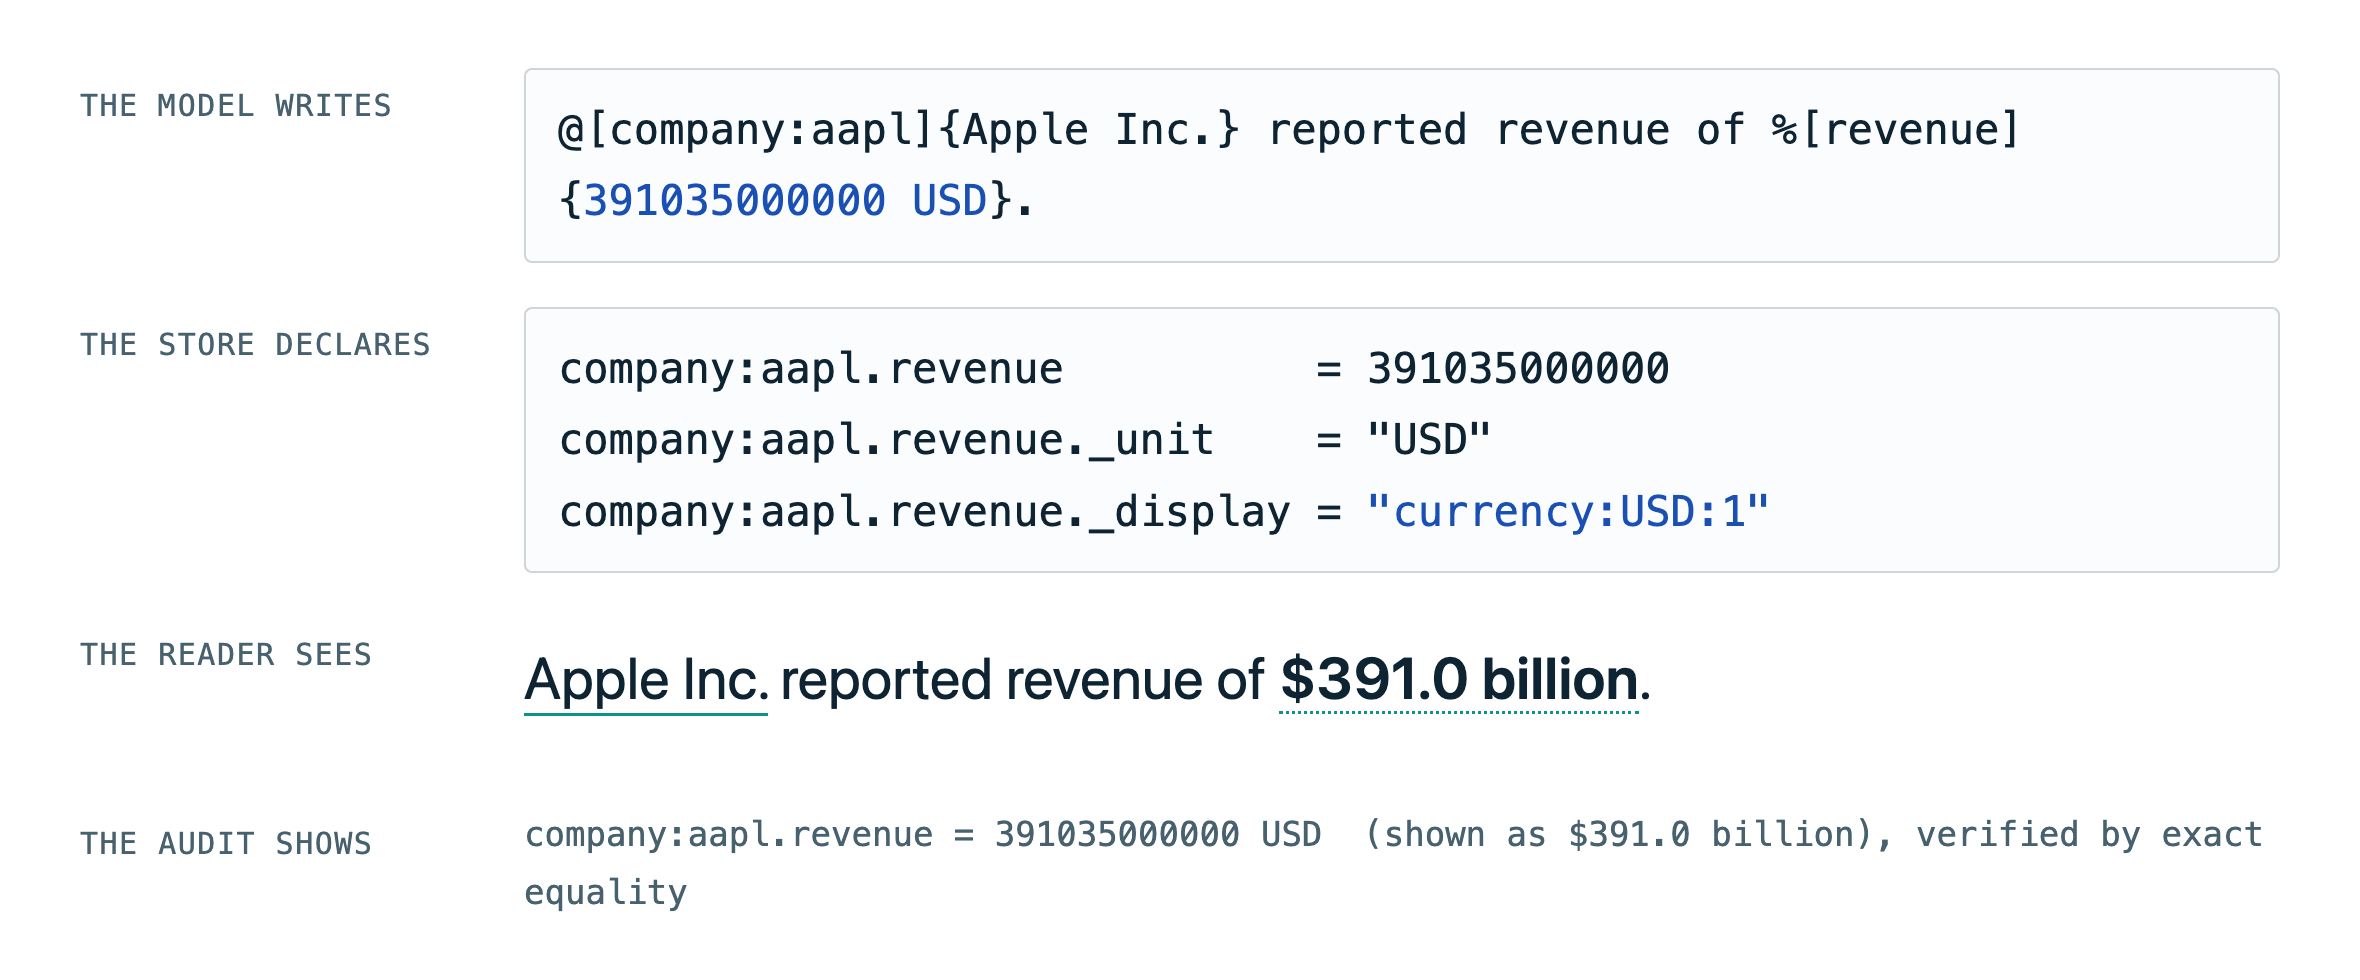
\includegraphics[width=\textwidth]{fig-display.png}
\caption{One claim, three views. The model writes the canonical value; the store declares the unit and a display rule next to the field; the reader sees the rounded form; the audit view keeps the exact value and says how it was shown. The model never rounds, so it can never round wrong.}
\label{fig:display}
\end{figure}

\paragraph{The threshold registry} follows a pattern shared by clinical reference intervals, JSON Schema validation and monitoring alert rules: a bounded condition on a single field is given a name and a human-readable label, so the judgment can be invoked and audited by that name rather than restated as an expression wherever it is used \citep{ozarda2016,jsonschema2022,prometheusalerting}. Each definition has a name, a field, one predicate from a deliberately small vocabulary (Table~\ref{tab:operators}), an optional unit constraint, a label and a source for audit:

\begin{lstlisting}
IS_LOW:        score lt 25         "critically low"
IS_MODERATE:   score between 25 50 "moderate"
IS_ACTIVE:     status in {A,B,C}  "active"
IS_MISSING:    value is_null       "no data"
MUCH_HIGHER:   _scoreDiff diff_gt 20 "much higher"
IS_NEGATIVE:   balance lt 0 [EUR]  "negative balance"
\end{lstlisting}

\begin{table}[h]
\centering
\small
\begin{tabular}{lll}
\toprule
\textbf{Operator} & \textbf{Display label} & \textbf{Example} \\
\midrule
\multicolumn{3}{l}{\textit{Core (numeric comparison)}} \\
\texttt{lt} & is less than & \texttt{price lt 10} \\
\texttt{lte} & is at most & \texttt{rating lte 3} \\
\texttt{gt} & is greater than & \texttt{stock gt 0} \\
\texttt{gte} & is at least & \texttt{score gte 75} \\
\texttt{eq} & equals & \texttt{status eq "active"} \\
\texttt{neq} & is not & \texttt{status neq "archived"} \\
\texttt{between} & is between & \texttt{score between 25 50} \\
\midrule
\multicolumn{3}{l}{\textit{Extended}} \\
\texttt{in} & is one of & \texttt{category in \{A,B,C\}} \\
\texttt{is\_null} & is missing & \texttt{value is\_null} \\
\texttt{diff\_gt} & exceeds by more than & \texttt{\_scoreDiff diff\_gt 20} \\
\bottomrule
\end{tabular}
\caption{Threshold operator vocabulary. Core operators cover numeric comparison and ranges. Extended operators handle categorical data, missing values, and cross-entity comparison.}
\label{tab:operators}
\end{table}

\paragraph{Verification} resolves each construct against the store --- string equality for entities and facts, typed comparison for thresholds --- with no model in the loop, so it is exact, explainable and effectively free (Section~\ref{sec:deployment}). A judgment the verifier cannot evaluate, because the threshold it names was never registered or the value it needs is missing, is reported as unverifiable, and negating it does not make it verified: \texttt{NOT} of an unverifiable condition is still unverifiable. Without that rule a model could get a claim past the verifier by negating a threshold that does not exist. Because errors come back as specific messages (``\texttt{\%[passRate]\{7\} in student:42: should be 5}''), verification can sit inside a generation loop that feeds each error back to the model; and because the verifier only reads the text, it can equally audit text it did not generate. A verification rate counts only what is inside markup, so a text that marks one number and leaves nine in prose would score 100\%; the verifier therefore also reports \textit{coverage}, the share of standalone numbers that sit inside a claim (years, list markers and code excluded), and in strict mode treats each number outside one as a finding. Figure~\ref{fig:comparison} shows the pipeline; Figure~\ref{fig:render-audit} the audit rendering, where each claim carries its proof path. The complete grammar is in Appendix~\ref{app:grammar}; Appendix~\ref{app:formal} states the semantics and the properties the mechanised model proves for it.

\begin{figure}[h]
\centering
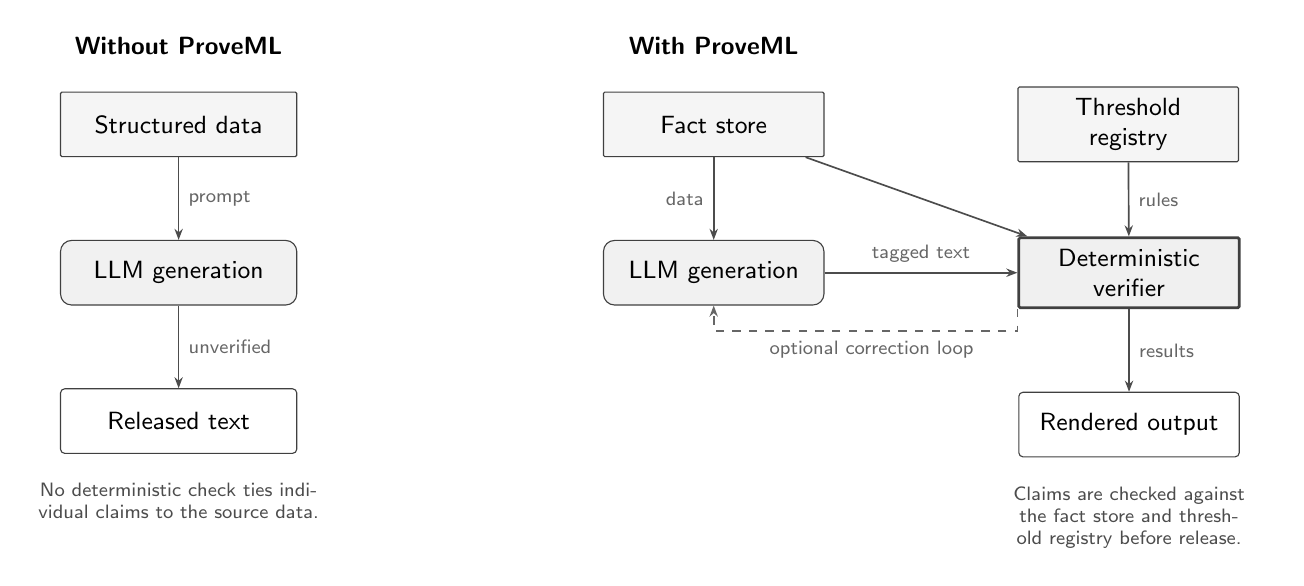
\begin{tikzpicture}[
    node distance=1.05cm and 1.55cm,
]
% Without ProveML
\node[diag title] (t1) {Without ProveML};
\node[diag data, below=0.35cm of t1, minimum width=3.0cm] (db1) {Structured data};
\node[diag ai, below=of db1, minimum width=3.0cm] (llm1) {LLM generation};
\node[diag out, below=of llm1, minimum width=3.0cm] (out1) {Released text};
\draw[diag arrow] (db1) -- (llm1) node[diag label, midway, right] {prompt};
\draw[diag arrow] (llm1) -- (out1) node[diag label, midway, right] {unverified};
\node[diag note, below=0.25cm of out1, text width=3.6cm] {No deterministic check ties individual claims to the source data.};

% With ProveML
\node[diag title, right=4.15cm of t1] (t2) {With ProveML};
\node[diag data, below=0.35cm of t2, minimum width=2.8cm] (fs2) {Fact store};
\node[diag data, right=2.45cm of fs2, minimum width=2.8cm] (tr2) {Threshold\\registry};
\node[diag ai, below=1.05cm of fs2, minimum width=2.8cm] (llm2) {LLM generation};
\node[diag det, right=2.45cm of llm2, minimum width=2.8cm] (ver2) {Deterministic\\verifier};
\node[diag out, below=1.05cm of ver2, minimum width=2.8cm] (ren2) {Rendered output};
\draw[diag arrow] (fs2) -- (llm2) node[diag label, midway, left] {data};
\draw[diag arrow] (fs2) -- (ver2);
\draw[diag arrow] (tr2) -- (ver2) node[diag label, midway, right] {rules};
\draw[diag arrow] (llm2) -- (ver2) node[diag label, midway, above] {tagged text};
\draw[diag arrow] (ver2) -- (ren2) node[diag label, midway, right] {results};
\draw[diag feedback] (ver2.south west) -- ++(0,-0.28) -| (llm2.south) node[diag label, pos=0.24, below] {optional correction loop};
\node[diag note, below=0.25cm of ren2, text width=3.5cm] {Claims are checked against the fact store and threshold registry before release.};
\end{tikzpicture}
\caption{Without ProveML (left): data goes in, text comes out, no verification. With ProveML (right): every claim is checked against the fact store and threshold registry, with an optional correction loop. Rounded boxes denote generative components; squared boxes denote data stores and deterministic processing.}
\label{fig:comparison}
\end{figure}

\begin{figure}[h]
\centering
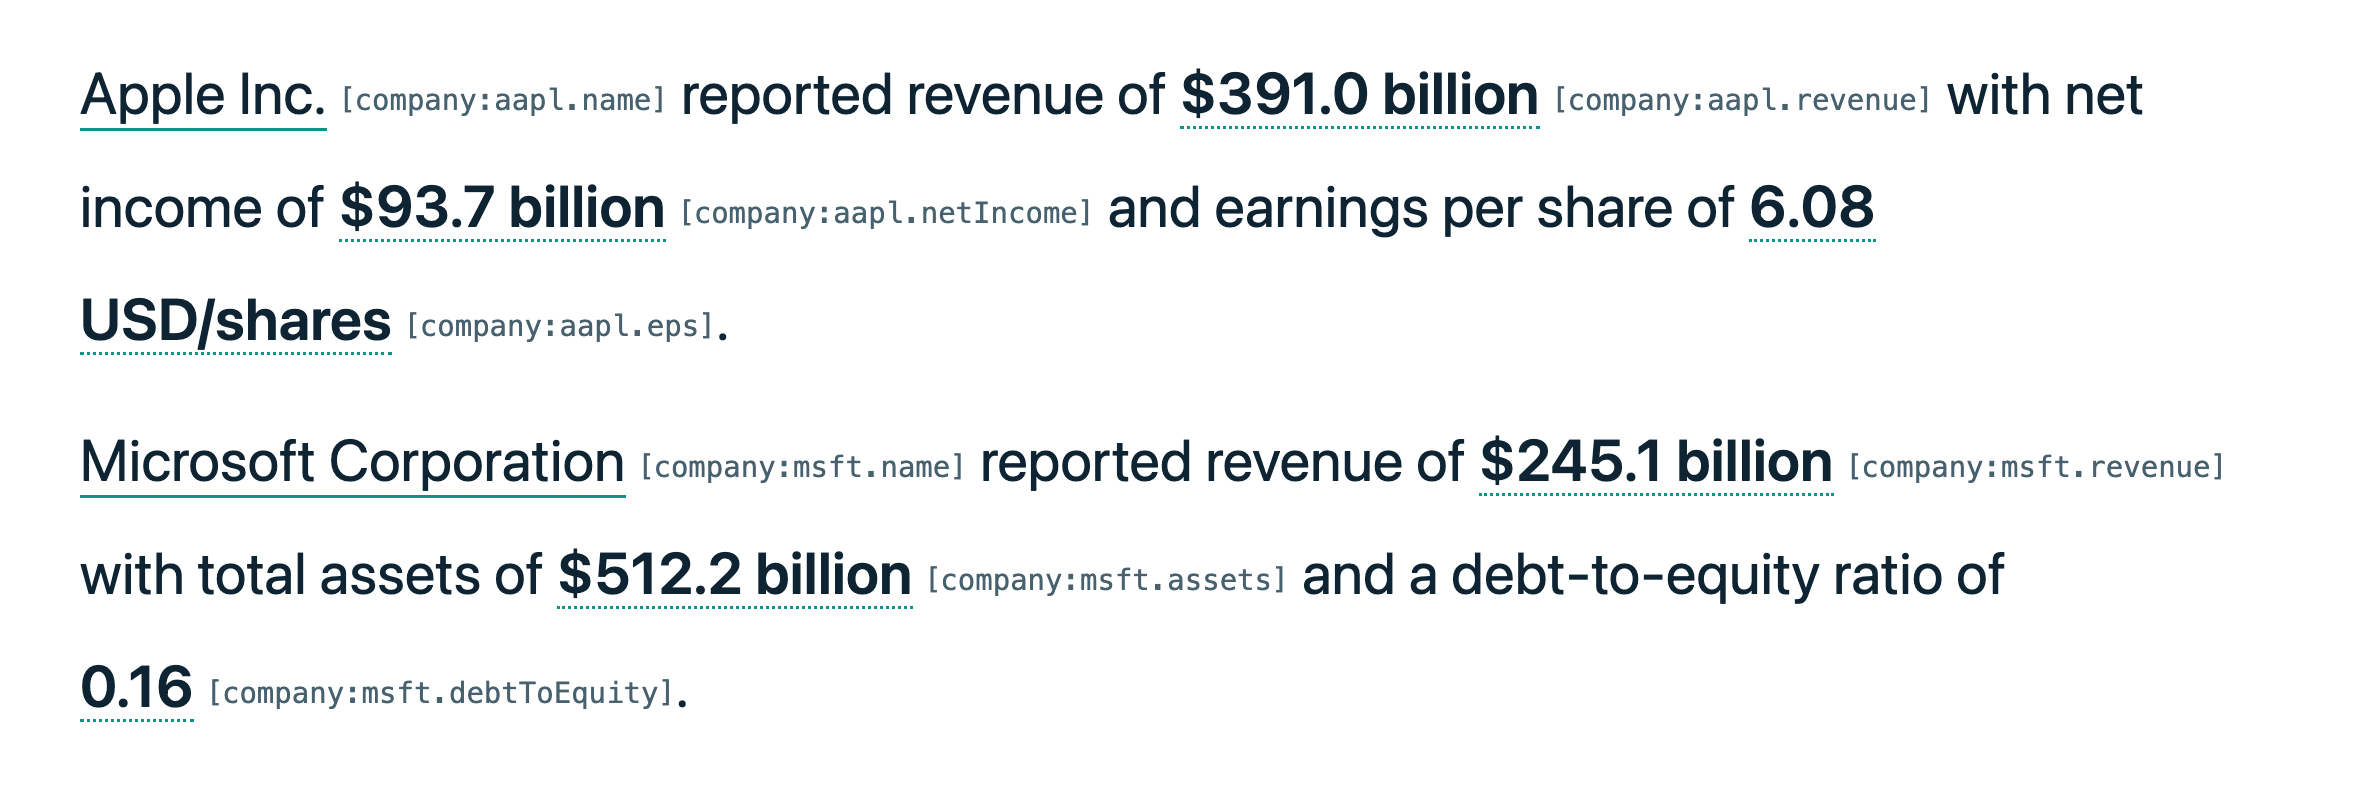
\includegraphics[width=\textwidth]{fig-audit-mode.png}
\caption{Audit mode: the fact-store path checked for each claim is visible inline (\texttt{company:aapl.revenue}, \texttt{company:msft.debtToEquity}). A reader, or an auditor months later, can take any number back to its record without a model.}
\label{fig:render-audit}
\end{figure}

\section{What We Measured}
\label{sec:evaluation}

\paragraph{Setup.} Three models that were frontier at the time of writing (August 2026): Claude Opus 5 and Claude Sonnet 5 (Anthropic, through the Claude Code CLI with default settings), and DeepSeek V4 Pro (\texttt{DeepSeek-V4-Pro-0813}, open weights under MIT, served by Together AI). Two benchmarks: 28 English prompts over a generated educational dataset of 741 pupils in 95 class offerings,\footnote{Generated, not de-identified: every record is drawn from a latent-ability model, the school is fictional, and the seeded generator ships with the artifacts. We state this from experience: an earlier draft used a de-identified extract of real records under the label ``synthetic''; it was withdrawn, replaced, and every educational result re-measured on the replacement.} and 10 English prompts over real SEC EDGAR FY2025 filings (2 entities, 11 fields). Three runs per model and benchmark, one correction pass: the verifier's errors are fed back once, and the corrected answer is accepted only if it verifies better without dropping claims. Verification rate is a per-query macro-average; a response with no markup scores 0\%, an empty answer scores 0\% rather than being dropped. Context is sliced per prompt from the benchmark's own entity lists --- an oracle retriever, which makes the rates an upper bound conditional on retrieval. The system prompt asks for entity and fact markup; no run produced an inference construct, so all rates measure those two. Every number in this section regenerates from the published runs (\texttt{experiments/frontier-summary.mjs}, \texttt{frontier-residuals.mjs}); the verifier's own conformance test (20 planted errors, all caught) is in Appendix~\ref{sec:detection}.

\begin{table}[h]
\centering
\small
\begin{tabular}{llcccc}
\toprule
\textbf{Benchmark} & \textbf{Model} & \textbf{First pass} & \textbf{One correction} & \textbf{Fully verified} & \textbf{Coverage} \\
\midrule
Education & Claude Opus 5 & 86.5\% $\pm$ 0.3 & 94.8\% $\pm$ 4.8 & 23.3/28 & 91.4\% \\
 & Claude Sonnet 5 & 89.3\% $\pm$ 2.1 & 92.2\% $\pm$ 3.6 & 21.3/28 & 92.3\% \\
 & DeepSeek V4 Pro & 97.2\% $\pm$ 1.3 & 99.5\% $\pm$ 0.8 & 27.7/28 & 94.2\% \\
\midrule
Finance & Claude Opus 5 & 97.9\% $\pm$ 0.6 & 100\% $\pm$ 0.0 & 10/10 & 95.8\% \\
 & Claude Sonnet 5 & 96.5\% $\pm$ 1.2 & 96.5\% $\pm$ 1.2 & 7/10 & 89.8\% \\
 & DeepSeek V4 Pro & 100\% $\pm$ 0.0 & 100\% $\pm$ 0.0 & 10/10 & 96.4\% \\
\bottomrule
\end{tabular}
\caption{Three frontier models, three runs each (mean $\pm$ sample sd over runs). First pass and after one correction: per-query verification rate. Fully verified: queries on which every claim verified after at most one correction (mean over runs). Coverage: numbers inside a claim as a share of all standalone numbers in the delivered text, pooled over runs, by the verifier's own definition.}
\label{tab:frontier}
\end{table}

\paragraph{Finding 1: the mechanism is within reach of current models.} No model, on any of the 342 query-runs, produced an empty answer or an answer without markup, and no call failed. First-pass verification runs from 86.5\% to 100\%, coverage from 89.8\% to 96.4\%, and one correction pass lifts Opus 5 by eight points on education and closes finance entirely (Table~\ref{tab:frontier}). The open-weight model is the strongest of the three on both benchmarks, at a third of the latency (3.4\,s per query against 7.9 and 11.8\,s, Section~\ref{sec:deployment}). Rate and coverage move together here, unlike in the earlier study of small models, where they diverged by more than thirty points at identical rates (technical report): at the frontier, a model that marks up reliably also marks up nearly everything.

\paragraph{Finding 2: what remains is mostly the binding rule, not the model.} Of the 157 errors still standing after the correction pass on the educational benchmark, 108 (69\%) have one shape. The sentence names the pupil and then the class --- \textit{``@[student:20414]\{Amir Janssens\} of @[offering:10056]\{5OL\} has a pass rate of \%[passRate]\{53\}\%''} --- and linear carry-forward binds the pupil's facts to the class, the nearest preceding entity. The data is right, the English is right, and the verifier reports \texttt{offering:10056.passRate} not found. It touched 17 of the 35 non-converged query-runs, and the correction pass could not repair it because nothing in the error message says which entity the fact should have gone to. The scoped form exists for exactly this, and no model used it. We have therefore made a fact able to name its own record, \texttt{\%[student:20414.passRate]\{53\}}, which the grammar's \texttt{path\_field} production always admitted and the verifier now honours, and then measured it (Finding 3). Wrong values are 40 of the 157 (25\%), almost all on aggregation prompts that ask for a rank or a count the store does not hold. Two errors are a bound written as a fact (\texttt{\%[passRate]\{60\}} before any entity, for ``a 60\% threshold''): a number that is not a record, which is what the inference construct is for.

\begin{table}[h]
\centering
\small
\begin{tabular}{llcccc}
\toprule
\textbf{Benchmark} & \textbf{Model} & \textbf{First pass} & \textbf{One correction} & \textbf{Fully verified} & \textbf{Coverage} \\
\midrule
Education & Claude Opus 5 & 95.4\% $\pm$ 7.5 & 97.1\% $\pm$ 4.7 & 25.7/28 & 97.9\% \\
 & Claude Sonnet 5 & 99.4\% $\pm$ 0.2 & 99.4\% $\pm$ 0.2 & 25.7/28 & 91.1\% \\
 & DeepSeek V4 Pro & 99.2\% $\pm$ 1.5 & 100\% $\pm$ 0.0 & 28/28 & 95.1\% \\
\midrule
Finance & Claude Opus 5 & 100\% $\pm$ 0.0 & 100\% $\pm$ 0.0 & 10/10 & 98.2\% \\
 & Claude Sonnet 5 & 100\% $\pm$ 0.0 & 100\% $\pm$ 0.0 & 10/10 & 94.4\% \\
 & DeepSeek V4 Pro & 100\% $\pm$ 0.0 & 100\% $\pm$ 0.0 & 10/10 & 97.6\% \\
\bottomrule
\end{tabular}
\caption{The same study under the second prompt, which adds two rules to the first: a fact may name its own record when the sentence names two subjects, and a cutoff from the question is not a fact. Everything else --- models, benchmarks, slices, runs, correction budget --- is identical to Table~\ref{tab:frontier}.}
\label{tab:frontier2}
\end{table}

\paragraph{Finding 3: told the rule, the models follow it, and the residue goes.} We re-ran the study with two sentences added to the system prompt, the binding rule and the cutoff rule, and nothing else changed (Table~\ref{tab:frontier2}). On finance all three models verify every claim on the first pass in every run. On education Sonnet 5 rises from 89.3\% to 99.4\%, DeepSeek from 97.2\% to 99.2\% and to 100\% after one correction, and Opus 5 from 86.5\% to 95.4\%: two of its three runs verify 100\% of claims on the first pass, and in the third it reverted, on three pupil queries, to the very phrasing the rule addresses (``Ali Peeters of 6WEWI has a pass rate of \ldots'') without the explicit record, which accounts for the spread. The 108 binding errors of the first study are 16 in the second, all in that one run. What remains elsewhere is small and mixed: a handful of wrong aggregates, and a model asking for a field the store does not hold (\texttt{passRateDiff}, \texttt{unevaluatedCount}) rather than inventing a number for it, which is the failure the design prefers. The rules now ship with the implementation as a generated system prompt (\texttt{proveml/prompt}), built from the store and the registry so the names the model sees are the names the verifier resolves; each rule in it is tied to a measured gap, and this is how we expect the prompt to evolve.

\paragraph{A first pass of this study measured the harness.} The context handed to the models named the fields \texttt{students} and \texttt{rate} where the store held \texttt{studentCount} and \texttt{passRate}. Every model reproduced what it was shown, and those two names were the two most frequent ``field not found'' errors of that pass. We record it because the same mismatch was present in the July 2026 study, whose residual-error analysis it inflated, and because it is a general lesson for deployments: the vocabulary the model sees must be the vocabulary the store resolves, or addressability errors will be measured that no model made.

\paragraph{The third construct: judgments.} The two studies above asked for entities and facts. A third study, run in September 2026, asks for the judgment construct. Twenty questions over the education store invite a qualitative assessment and name no cutoff (``How is 6VZ doing?'', ``Is 6ZW a strong class?'', ``Why is 6VZ doing so badly?'', ``Is 3BS's teacher effective?''): eight that the data supports, four at a registered bound (6ZW at a pass rate of 74 against \texttt{IS\_STRONG} at 75 or more; a pupil with 29 absences against \texttt{IS\_GREY\_RISK} above 30), four that presuppose a judgment the data refutes, and four that invite a judgment no registry entry covers. The registry is the education part of the example registry that ships with the package, fourteen names selected by field, and the prompt is the one \texttt{proveml/prompt} generates from the store and that registry. The same questions ran under the facts-only prompt of the studies above as the baseline. Same three models, three runs each, one correction pass. Which registered conditions hold for each record in a question's context is computed by the verifier and saved with the run, so the boundary and contrary questions score themselves.

\begin{table}[h]
\centering
\small
\setlength{\tabcolsep}{3pt}
\footnotesize
\begin{tabular}{lccccc}
\toprule
\textbf{Model} & \textbf{Responses} & \textbf{Judgments} & \textbf{First pass} & \textbf{One correction} & \textbf{Boundary, contrary} \\
\midrule
Claude Opus 5 & 20/20 & 67.7 $\pm$ 5.5 & 92.6\% $\pm$ 1.1 & 100\% $\pm$ 0.0 & 7.3 $\to$ 8.0 of 8 \\
Claude Sonnet 5 & 19.3/20 & 42.3 $\pm$ 4.2 & 77.8\% $\pm$ 3.3 & 98.2\% $\pm$ 1.5 & 3.7 $\to$ 7.7 of 8 \\
DeepSeek V4 Pro & 18.0/20 & 41.3 $\pm$ 1.2 & 100\% $\pm$ 0.0 & 100\% $\pm$ 0.0 & 8.0 $\to$ 8.0 of 8 \\
\midrule
Without a registry & 0/20 & 0 & \multicolumn{3}{l}{18 to 26 uncheckable qualitative words per run} \\
\bottomrule
\end{tabular}
\caption{The judgment study: 20 questions that invite a qualitative assessment, mean $\pm$ sample sd over three runs. Responses: those carrying at least one judgment. Judgments: emitted per run. First pass and one correction: the share of emitted judgments whose registered condition holds. Boundary, contrary: of the eight such questions, those on which no judgment the data refutes survived, before and after the correction. No model in any run named a threshold the registry does not hold.}
\label{tab:judgment}
\end{table}

\paragraph{Finding 4: models use the construct, never invent a name, and reach for the word the sentence wants.} With the registry every Opus 5 response, 19 of 20 Sonnet 5 responses and 18 of 20 DeepSeek responses carry at least one judgment: 454 judgments over nine runs, 411 of them verified on the first pass and 425 of 427 after one correction (Table~\ref{tab:judgment}). Without it, the same questions draw 18 to 26 qualitative words per run (strong, low, at risk, average, concern) that no verifier can see; that is the baseline this construct replaces. Not one of the 454 named a threshold outside the registry. On the four questions with no matching entry the models stated the numbers and said the data holds no such field, or used a registered judgment that holds; one correction on Sonnet 5 produced a malformed label, the single judgment left unverified. The 33 first-pass failures are almost all one thing: ``small sample'' at 5 or 7 pupils against a bound of 5, ``strong'' at 74 or 63 against 75, ``reliable sample'' at 7 or 8 against 10, ``risk of grey marks'' at 29 absences against 30. The model reached for the word the question invited, the registry's bound said no, and the correction removed the claim rather than the number. That is the overreach the registry exists to catch, and it is caught deterministically: on the eight boundary and contrary questions Sonnet 5 answered 3.7 of 8 soundly on the first pass and 7.7 after one correction, Opus 5 went from 7.3 to 8, DeepSeek was sound on all 8 in both. A second observation from the setup rather than the runs: an \texttt{is\_null} judgment is vacuously true on a record type that never carries the field, so \texttt{IS\_MISSING} on \texttt{evaluated} would have verified for every class; it was excluded, and the specification should say that a missing field is not a null value.

\section{Deployment}
\label{sec:deployment}

The evaluation measures whether models can produce verifiable markup. This section reports what it costs to run and what a deployment has to build, because both are load-bearing for anyone deciding whether to adopt the mechanism, and neither follows from the tables above.

\paragraph{Cost of verification: negligible next to generation.} Verifying the 2{,}185 claims in the 252 stored final responses of the educational runs against the 4{,}826-key fact store takes 0.66\,s on a laptop, mean of 20 passes --- 2.6\,ms per response, 0.30\,ms per claim (the script \texttt{deployment-numbers.mjs} in \texttt{experiments/}, run with \texttt{--tag frontier}, recomputes every figure in this section). The cost per claim grows with the store, because the verifier scans the store for each fact to establish that its subject is unique; an indexed store would bring it to microseconds, and an earlier version of this paper printed a microsecond figure that only holds on a toy store. Against generation latency (3.4 to 11.8\,s per query, summed over the correction pass) this is free, which is what allows verification to sit inside the generation loop rather than after it.

\paragraph{Cost of generation: markup and retries.} Two overheads are real. Marked-up responses ran 49\% (Opus 5), 66\% (Sonnet 5) and 79\% (DeepSeek) longer in characters than the same text with the markup stripped; the shortest answers pay the highest relative price, because the markup is a fixed cost per claim. That is a direct output-token cost. The correction pass adds a second: 77\% of query-runs needed none, and the mean is 1.23 generations per query (1.06 for DeepSeek, 1.33 for Opus 5). A deployment that allows one pass and no more captures what we measured; the July study found that further passes rarely change the outcome.

\paragraph{What a deployment has to build.} The fact store is the work. Flattening records into \texttt{type:id.field} is mechanical once the entities are decided, but deciding them is a modelling exercise: a normalized database with joins does not announce what counts as one addressable entity, and that choice determines which claims can be bound at all. Derived values are the recurring case --- a count, a difference, a ratio the report computes on the fly --- and the rule is that arithmetic belongs in the data layer, materialized as an addressable fact, rather than in the verifier (Section~\ref{sec:proveml}). A threshold registry is optional at the entity-and-fact level and small when present: the example registry that ships with the implementation has twenty-one entries, and neither benchmark needed one (no run produced an inference), so its cost falls entirely on the deployments that use it. The vocabulary the model is shown must be the store's vocabulary (Section~\ref{sec:evaluation}); that is a one-line rule and an easy one to break.

\paragraph{The retrieval assumption, stated plainly.} Our headline rates assume retrieval has already succeeded: context slices come from the benchmark's own entity lists, an oracle retriever. The July study's full-context ablation shows what happens without slicing for small models --- zero constructs on every query, with the numbers emitted as plain prose instead (technical report); we did not repeat it at the frontier. Context selection is a precondition of the mechanism, and its quality in a real deployment is the largest variable this paper does not measure. Treat the reported rates as an upper bound conditional on retrieval, and budget for the retrieval work accordingly.

\paragraph{Minimal integration.} The reference implementation is an npm package whose verifier has no runtime dependencies (only the optional markdown-it plugin needs a peer):

\begin{lstlisting}
import { verifyProveml } from 'proveml/verify';

const store = { 'student:42.name': 'Alex', 'student:42.passRate': 5 };
const text  = '@[student:42]{Alex} scored %[passRate]{5}%.';

const { verified, total, errors } = verifyProveml(text, store);
// -> 2 / 2, no errors
\end{lstlisting}

\noindent A deployment adds three things to an existing LLM call: the store, a system prompt that asks for the markup, and the verifier on the response. The verify-fix loop and the rendering layer are optional on top.

\paragraph{The store's own provenance.} The first limitation in Section~\ref{sec:limitations} --- verified means consistent with the store, not true --- marks the one link the verifier cannot close, and the implementation gives a deployment a discipline for it rather than leaving it to trust. In the review layer (\texttt{proveml/review}), every store value carries its evidence: a quote checked verbatim against an archived snapshot of its source, a declared derivation, or a declared absence, because one cannot quote a source not having something. The machine re-checks those links at build time and refuses to emit the review page when any fails; the one link it cannot check --- whether a value is a fair reading of its evidence --- is judged by a person on that page, and each judgement is saved under a hash of exactly what it judged, so it expires the moment the evidence changes and review shrinks to the diff. The gate is awaitable in a pipeline (\texttt{proveml review --await} exits nonzero while readings are unjudged or flagged), and how a sign-off is attested is an adapter, so a deployment can bind it to a name, a key signature, or a ledger anchor. This paper applies the layer to itself: its related-work characterisations are ProveML claims against a citation store whose evidence readings ran through exactly this page, quote by quote.

\section{Related Work}
\label{sec:related}

The idea of tagging human-readable text for machine resolution is old: RDFa binds spans of prose to entities in a structured vocabulary and assumes the author meant it \citep{rdfa}; iXBRL embeds machine-readable tags in financial reports for automated audit \citep{ixbrl}. ProveML adds the verdict to that lineage --- not what a span refers to, but whether the claim survives comparison with the record. Among recent systems, Proof-Carrying Numbers \citep{pcn2025} is the nearest neighbor (claim-bound numeric tokens, deterministically verified in the renderer, with declared tolerance policies; its published description does not cover entity scoping or a named vocabulary for qualitative judgments), and SymGen \citep{symgen} takes the opposite strategy: the model emits references and a parser substitutes the values, so a wrong number is impossible and so is reporting one; the technical report compares the two on identical runs. Claim-locked reporting \citep{claimlocked2026} is the 2026 form of that strategy --- the numbers, their direction and the permitted strength of language are fixed before the model writes connective prose --- and shares ProveML's premise that qualitative wording must be tied to a declared threshold, while giving up the ability to audit text it did not produce. VeriFin \citep{verifin2026} checks financial claims against XBRL facts with an SMT solver, placing the arithmetic in the verifier where ProveML places it in the data layer. \citet{datareferencing2026} measure the failure class our residual errors belong to --- values miscited from a table the model was shown --- and detect it with a trained critic; ProveML detects it with a lookup. Fact verification against evidence has a canonical benchmark lineage --- FEVER \citep{fever}, TabFact \citep{tabfact}, FEVEROUS \citep{feverous} --- in which a trained model judges support; ProveML sits outside it by making the judgment a lookup. Probabilistic faithfulness checkers, academic (SummaC, \citealp{summac}; AlignScore, \citealp{alignscore}; MiniCheck, \citealp{minicheck}; HallDetect, \citealp{halldetect2026}) and industrial, score responses after generation; Evergreen \citep{evergreen2026} verifies aggregate claims over relational data as queries, which ProveML can only bind once the aggregate is materialised as a fact; structured inline citation \citep{fullcite2026} and decode-time grammars whose reference slots admit only declared names \citep{dtg2026} are the constrained-generation route to the same end, and the natural next step for ProveML (Section~\ref{sec:limitations}). To our knowledge, no existing framework combines inline claim markup, deterministic mismatch detection against structured data, and composable threshold inference in a single system.\footnote{We screened the titles and abstracts of the 4{,}617 papers in the ACL 2026 main, short, findings and industry volumes against concept patterns for claim-level attribution, structured-data faithfulness, symbolic or deterministic verification, provenance and markup schemes, then read the resulting candidates by hand. The sweep was not preserved as a runnable artifact, so this is the result of a search rather than an exhaustive negative.} Table~\ref{tab:related} places the neighbours; the technical report discusses each in full.

\begin{table}[h]
\centering
\small
\begin{tabular}{llcccc}
\toprule
\textbf{Approach} & \textbf{Category} & \textbf{Determ.} & \textbf{Structured} & \textbf{Inline} & \textbf{Inference} \\
\midrule
FActScore, SAFE, FacTool, HallDetect & Fact-checking & -- & -- & -- & -- \\
Guardrail and grounding scorers & Guardrails & -- & -- & -- & -- \\
Schema validators, decode-time grammars & Schema & \checkmark & -- & -- & -- \\
ClaimDB, Evergreen, VeriFin & Data-grounded & \checkmark & \checkmark & -- & -- \\
FullCite & Inline citation & -- & -- & \checkmark & -- \\
iXBRL$^*$ & Inline tagging & \checkmark & \checkmark & \checkmark & -- \\
SymGen & Inline tagging & \checkmark & \checkmark & \checkmark & -- \\
PCN & Inline tagging & \checkmark & \checkmark & \checkmark & -- \\
Claim-locked reporting & Inline tagging & \checkmark & \checkmark & \checkmark & Partial \\
FinGround & Hybrid post-hoc & Partial & \checkmark & -- & -- \\
\textbf{ProveML} & \textbf{Inline tagging} & \checkmark & \checkmark & \checkmark & \checkmark \\
\bottomrule
\end{tabular}
\caption{Comparison across representative verification approaches. Determ.\ = deterministic. Structured = against structured data. Inline = claim-level markup in text. Inference = composable threshold checks within natural language text. The guardrails row reflects the predominant model-based grounding mode, in which a trained model scores a response against its source and a threshold decides the outcome (Amazon Bedrock Guardrails contextual grounding check \citep{bedrockgrounding2026}, Azure AI Content Safety groundedness detection \citep{azuregroundedness2026}, Vectara's HHEM \citep{vectarahhem2026} and similar); Amazon Bedrock's separate Automated Reasoning checks add formal logic checks against a declared policy and validate only what the policy's variables capture, not author-marked claims in the text \citep{bedrockautoreasoning2026}. Claim-locked reporting ties language strength to statistical thresholds but does not compose them. FinGround recomputes arithmetic claims deterministically but decomposes and types them with a model, hence Partial. $^*$The XBRL formula family provides document-level computation and assertion checks over the facts in a report \citep{xbrlvalidation2009,xbrlvalueassertions2009}; the Inline XBRL specification is scoped to syntax and to mapping it into an XBRL instance, and defines no claim-scoped inference \citep{ixbrl}.}
\label{tab:related}
\end{table}

\section{Discussion and Limitations}
\label{sec:limitations}

The deeper value is not the correction loop but the boundary itself. With ProveML markup, every marked claim carries a verification status and an addressable path, so a reader --- or an auditor months later --- can ask of any number where it came from and get an answer that does not depend on a model. What changes is the unit of accountability: from ``was this report right'' to ``was this claim right, and against which record''. Because entity references are structural and display text is separate from the identifier the verifier resolves, a deployment can hand the model pseudonymous identifiers and substitute names at display time --- a property the syntax makes available, not one we evaluated.

\begin{itemize}[nosep]
    \item \textbf{Consistency, not truth.} ProveML verifies that claims match the fact store, not that the fact store is correct. If the source data is wrong, verified claims will be wrong. The review layer described under Deployment gives that boundary a discipline --- evidence per store value, a human sign-off saved under a hash of exactly what it judged, expiring when the evidence changes --- but does not remove it: a fair reading is a judgement, not a proof.
    \item \textbf{The right name, not necessarily the right record.} An entity verifies when the name the reader sees equals the name stored at the id the model chose; nothing checks that the model chose the right id. If two records of one type share a name, a wrong id renders identically to the right one and only the audit path tells them apart. The verifier therefore measures whether a rendered subject is unique in the store (\texttt{subjectUnique}: true, false with the other paths, or unknown when the source cannot be enumerated), \texttt{doctor} warns on duplicate names, strict mode makes an ambiguous subject a finding, and the render marks it. Where subjects are identifiers by construction, as on a ledger, the gap closes; where they are personal names, it does not, and the marker is what remains.
    \item \textbf{No unit conversion.} Units are supported as nullable metadata with exact string matching. Semantic unit equivalence (e.g., mg/dL vs mmol/L) and standardized vocabularies (UCUM for units of measure~\citep{ucum}, ISO 4217 for currency codes~\citep{iso4217}) are deferred to future work.
    \item \textbf{Evaluation scope.} The evaluation covers two domains (generated education, real SEC finance) across 38 prompts, 3 models, and 3 repeats, with an oracle retriever and one correction pass. Larger schemas, more domains, and retrieval under realistic conditions are not covered. The explicit-record fact form was introduced after the first study and measured in the second (Finding 3); whether a model follows the rule on every run is not guaranteed, as one Opus 5 run shows.
    \item \textbf{Judgments: one domain, one registry.} The judgment study covers one store, one registry of fourteen names and twenty questions, and its baseline is the facts-only prompt rather than free prose. How the construct behaves with a large registry, with judgments over derived values, or when the registry itself is contested, is not measured.
    \item \textbf{Canonical claims.} The model is not allowed to round: a claim says \texttt{391035000000}, never ``\$391 billion''. The reader can still see the rounded form, because the store may declare a display rule per field (\texttt{\_display}) that the renderer applies to verified values; but a value the model itself rounded is a mismatch, and prose that quotes the rounded figure outside a claim is unverified prose. The rule is on the store's side of the boundary on purpose: a tolerance in the verifier would make ``about 18'' verify against 18.5 and turn the guarantee into an approximation.
    \item \textbf{Prose outside markup.} ProveML verifies what is inside markup constructs. Text outside the markup is not checked. The verifier now measures the numeric part of this gap as coverage (90--96\% in Section~\ref{sec:evaluation}) and can refuse a number outside any claim, but a qualitative sentence with no number in it remains invisible to it. And a set of verified claims does not verify the sentence around them: \citet{chan2026soundness} argue that formally sound conclusions invite unsupported inferences by the reader, and nothing in ProveML's verdict speaks to what the prose between two verified claims implies.
    \item \textbf{Malformed input.} The tokenizer silently skips constructs with unmatched brackets or braces. Robustness to diverse malformed markup deserves further stress-testing.
    \item \textbf{Adversarial generation.} ProveML is designed against models that make mistakes, not against a model trying to mislead. A generator that wanted to could choose a threshold that holds and wrap misleading words around it, mark only the claims that verify and leave the damaging ones as prose, or select a true fact that misrepresents the record it came from. Each of these survives verification because the verifier reads paths and values, not intent. We neither measure nor defend against this.
    \item \textbf{Group claims.} Inferences evaluate against a single entity context. A claim like ``5TW, 4B, and 6WE all have low coverage'' cannot be verified as one inference; it must be decomposed into one inference per entity.
\end{itemize}

\noindent Future work follows from the limits: derived-value claims, standardized unit vocabularies, an abstention metric for unsupported queries, and constraining decoding to well-formed ProveML with only existing paths --- grammar-constrained generation (PICARD, \citealp{picard}; Synchromesh, \citealp{synchromesh}) makes that an application of known technique rather than a research program, and it would remove much of what we measure as addressability error.

\section{Conclusion}

ProveML places AI-generated claims inside a verifiable boundary. Three inline constructs link every claim to an addressable path in a data source. Verification is deterministic, with no model in the loop. An optional threshold registry extends this to qualitative judgments through composable primitives.

The evaluation (Section~\ref{sec:evaluation}) says that the mechanism is within reach of current models: three frontier models produce the markup on every query, cover 90--96\% of their numbers with claims, and verify 92--100\% of those claims after one correction. What remained was a property of the language more than of the models; the specification changed in response, and with the change in the prompt the residue went where the rule was followed. The earlier study of small local models (technical report) says the complement: below the frontier, whether a model produces verifiable markup at all depends on the shape of the request more than on the size of the model.

What LLMs provide is open-ended generation. What ProveML adds is a controllable, auditable boundary around that generation. For humans, the intended benefit is visual triage: verified claims carry a status, and attention shifts to what is unverified. We have not measured whether this reduces human verification effort, and the evidence from adjacent systems is mixed: \citet{symgen} report their user study reduced average verification time by 20\%, while \citet{ten2026} report a 21-participant study in which verification and correction effort did not differ significantly from their baseline, even though their system reduced hallucination. Which of the two ProveML's rendering resembles in practice is an open empirical question. For agent loops the benefit is more direct and does not depend on human factors: specific error feedback (``\texttt{\%[glucose]\{143 mg/dL\} in patient:308: should be 142 mg/dL}'') enables targeted self-correction, which is what the verify-fix loop measures in Section~\ref{sec:evaluation}. The combination is what neither open-ended generation nor static verification offers alone: open-endedness with determinism.

\section*{Declaration of Generative AI Use}

Generative AI tools (Claude, GPT) were used during manuscript preparation for drafting, revision, literature search, and code review. All AI-generated content was reviewed, verified, and edited by the author. No generative AI was used to create or alter images or artwork. The author takes full responsibility for the content of the published article.

\bibliographystyle{plainnat}
\bibliography{proveml}

\appendix

\section{Error Detection Rate}
\label{sec:detection}

\paragraph{Setup.} The critical question for ProveML is not whether the LLM generates correct output, but whether ProveML \textit{detects} incorrect output. To test this, we injected 20 deliberate errors into otherwise valid ProveML text and measured whether the verifier caught each one.

\paragraph{Results.} The 20 errors span six categories: wrong values (5), wrong entity (3), no context (2), wrong threshold (4), cross-entity swaps (2), and subtle errors including trailing spaces and swapped entity order (4). ProveML detected all 20, yielding a \textbf{100\% error detection rate}. This is a consequence of deterministic equality checking: if the claimed value does not exactly match the fact store, the claim is flagged regardless of plausibility. The experiment validates that the implementation behaves as specified --- it is a conformance test, not a detector benchmark --- and it is one-sided: it measures detection of planted errors, not false positives on correct-but-reformatted values (a canonicalization difference such as \texttt{18.50} vs.\ \texttt{18.5} is flagged despite numeric equality; see Section~\ref{sec:limitations}). Robustness to malformed LLM markup is partially addressed by the correction-loop results in Section~\ref{sec:evaluation} but deserves further stress-testing.

\section{Formal Semantics}
\label{app:formal}

This appendix states what the verifier computes, as definitions, and what the paper claims for it, as propositions. The definitions and the proofs are mechanised in Lean~4 in the artifact repository (\texttt{formal/}, no dependencies beyond Lean); every proposition below names its theorem there. The mechanisation models the judgment, which verdict a construct receives, not the tokenizer that turns text into constructs; that link is covered by test vectors the model prints and the reference implementation must reproduce (\texttt{formal/check-vectors.mjs}, 11 of 11 agree).

\paragraph{Verdicts.} A condition takes one of three values, $\mathbf{t}$, $\mathbf{f}$ or $\mathbf{u}$ (unresolved). The connectives are Kleene's strong three-valued logic: $\neg\mathbf{u}=\mathbf{u}$; $\mathbf{f}$ wins a conjunction and $\mathbf{u}$ otherwise wins it; $\mathbf{t}$ wins a disjunction and $\mathbf{u}$ otherwise wins it. The information order puts $\mathbf{u}$ below both decided values: $a \sqsubseteq b$ iff $a=\mathbf{u}$ or $a=b$. All three connectives are monotone in it.

\paragraph{Store and registry.} A store $S$ is a partial function from paths \texttt{type:id.field} to values; a value is a number or a text. The surface value of a path, $\mathrm{surf}_S(q)$, is its value as text followed by the unit at $q$\texttt{.\_unit} when the store declares one. A registry $R$ is a partial function from names to thresholds $(\mathit{field}, \mathit{op}, \mathit{unit}?)$; the operators are those of Table~\ref{tab:operators}, with $\mathit{between}$ read as $\mathit{lo} \le v < \mathit{hi}$ and $\mathit{eq}$, $\mathit{neq}$, $\mathit{in}$ on the value's text. Numbers are a parameter with a decidable order; the model does not choose between integers and decimals.

\paragraph{An atom.} A named threshold $N$ in context $c$ (the entity in force, or none), with an optional explicit path $p$, evaluates as follows. If $R(N)$ is undefined, $\mathbf{u}$. Otherwise let $t=R(N)$ and let the path be $p$ if $p$ is given and addresses $t.\mathit{field}$, undefined if $p$ is given and addresses another field, and $c\texttt{.}t.\mathit{field}$ if no $p$ is given and $c$ is defined; if the path is undefined, $\mathbf{u}$. If $t.\mathit{op}$ is $\mathit{is\_null}$, the verdict is $\mathbf{t}$ iff $S$ has no value at the path. Otherwise, if $S$ has no value there, $\mathbf{u}$; if $t$ declares a unit and the store's unit at the path is absent or different, $\mathbf{u}$; if an ordering operator meets a text, $\mathbf{u}$; else the operator's truth value. A label reference $@\ell$ is the verdict recorded under $\ell$ earlier in the document, $\mathbf{u}$ if none. Text the condition grammar rejects, a bare comparison included, is $\mathbf{u}$.

\paragraph{A document.} The tokenizer yields a sequence of constructs: an entity (path, rendered name, scoped or not), the close of a scope, a fact (a field of the entity in force, or an absolute path, and a value), or a judgment (label, condition). The verifier folds over the sequence with the entity in force, a stack of contexts, and the judgments so far by label. An entity becomes the entity in force and, if scoped, pushes the previous context, none included; a close pops it; a fact and a judgment leave the context as it is. Each construct receives one verdict: an entity is \emph{verified} iff the store's name at its id equals the rendered name; a fact is \emph{verified} iff its value equals the surface value at its path, \emph{no context} if it is relative and no entity is in force; a judgment is \emph{verified}, \emph{failed} or \emph{unverifiable} as its condition is $\mathbf{t}$, $\mathbf{f}$ or $\mathbf{u}$. Verification is a function of the document, the store and the registry, and of nothing else; determinism needs no proposition.

\paragraph{Propositions.} Write $S \sqsubseteq S'$ when every value $S$ holds, $S'$ holds; likewise $R \sqsubseteq R'$ for registries.

\begin{enumerate}[nosep]
    \item \textbf{Verified means equal to the store.} If the verifier reports a fact at path $q$ with value $v$ as verified, then $\mathrm{surf}_S(q)=v$; if it reports an entity at $p$ with name $n$ as verified, then $S(p\texttt{.name})$ is defined and reads $n$. There is no tolerance anywhere. (\texttt{verify\_fact\_sound}, \texttt{verify\_entity\_sound})
    \item \textbf{A verified judgment rests on a registered bound that holds.} If an atom evaluates to $\mathbf{t}$, its name is registered; and for every operator but $\mathit{is\_null}$, the store holds a value at the bound path, the unit the threshold asks for is present and equal, and the operator holds of that value. (\texttt{evalAtom\_tt\_registered}, \texttt{evalAtom\_tt\_holds})
    \item \textbf{Nothing unresolved contributes to a verdict.} If $R \sqsubseteq R'$ then for every condition, its verdict under $R$ is below its verdict under $R'$ in the information order: registering more names can decide an unresolved judgment and can never flip a decided one. In particular a verified judgment stays verified and a failed one stays failed when the registry grows, and against the empty registry every judgment is unresolved. This is the formal content of ``a model cannot make a claim checkable by naming a threshold the deployment never declared'', and $\neg\mathbf{u}=\mathbf{u}$ is what makes it hold. (\texttt{evalCond\_mono}, \texttt{evalCond\_tt\_stable}, \texttt{evalCond\_ff\_stable}, \texttt{evalCond\_empty})
    \item \textbf{Closing a scope restores the context in force when it opened.} For a scoped entity around a body that opens and closes no scope of its own, the context after the close equals the context before the entity. (\texttt{scope\_restores})
    \item \textbf{The store may grow too, with one exception.} If $S \sqsubseteq S'$ then an atom under any operator but $\mathit{is\_null}$ is below its verdict under $S'$. The exception is stated, not hidden: an $\mathit{is\_null}$ threshold evaluates to $\mathbf{t}$ wherever the store is silent, which includes a field the record's type never carries. That is the vacuity the judgment study met (Finding~4), and the specification should close it by distinguishing a missing field from a null value. (\texttt{evalAtom\_store\_mono}, \texttt{isNull\_vacuous})
\end{enumerate}

\paragraph{What this establishes and what it does not.} The propositions are about the model. The reference implementation is checked against it on the paper's examples, not proven to refine it; a verified implementation, the verifier written in the proof assistant and extracted, would close that gap and is the natural next step, and the tokenizer would then need modelling too. Beyond the mechanism nothing here is provable: that a verified claim is true is a property of the store, and that the text around it does not mislead is a property of the model. Both stay with the limitations in Section~\ref{sec:limitations}.

\section{ProveML Grammar (EBNF)}
\label{app:grammar}

The following EBNF captures the ProveML constructs as implemented in the reference parser. It is intended as a starting point for formal treatment, not a normative specification; the authoritative definition is the reference implementation and test suite. Where the two diverge, the reference tokenizer is deliberately \textit{more permissive} than this grammar --- for example, it accepts identifiers beyond the character classes below and tolerates a missing space after the inference label colon --- so the grammar describes the canonical surface form generators should produce, while the tokenizer accepts sloppier variants of it. One exception runs the other way: the tokenizer brace-counts entity display text, so an unbalanced open brace (admitted by the \texttt{display\_text} production) causes the construct to be skipped.

\begin{lstlisting}
(* ProveML constructs inside Markdown inline content *)
entity_ref_simple = "@[" , entity_path , "]{" , display_text , "}" ;
entity_ref_scoped = "@[" , entity_path , " " , DQUOTE ,
                    entity_name , DQUOTE , "]{" ,
                    scoped_content , "}" ;
entity_ref        = entity_ref_simple | entity_ref_scoped ;

fact_ref          = "%[" , field_name , "]{" , value_text , "}" ;
inference_ref     = "?[" , label , ": " , condition , "]{" ,
                    display_text , "}" ;

(* Paths and identifiers *)
entity_path       = identifier , ":" , entity_id ;
entity_id         = ( letter | digit ) ,
                    { letter | digit | "_" | "-" } ;

field_name        = field_segment , { "." , field_segment } ;
field_segment     = meta_field | path_field | identifier ;
meta_field        = "_" , identifier ;
path_field        = identifier , ":" , entity_id ;

label             = identifier ;
identifier        = letter , { letter | digit | "_" } ;

(* Text content *)
entity_name       = { char - '"' - ']' } ;
display_text      = { char - "}" } ;
scoped_content    = { char } ;   (* parsed recursively *)
value_text        = { char - "}" } ;

(* Condition grammar *)
condition         = or_expr ;
or_expr           = and_expr , { " OR " , and_expr } ;
and_expr          = unary_expr , { " AND " , unary_expr } ;
unary_expr        = [ "NOT " ] , primary ;
primary           = threshold_name
                  | threshold_name , "(" , path , ")"
                  | "@" , label ;

(* Terminals *)
threshold_name    = uppercase , { uppercase | digit | "_" } ;
path              = entity_path , "." , field_name ;
DQUOTE            = '"' ;
letter            = "a"-"z" | "A"-"Z" ;
uppercase         = "A"-"Z" ;
digit             = "0"-"9" ;
\end{lstlisting}

\end{document}
